\documentclass[a4paper, 14pt, oneside]{Thesis}
\usepackage{ulem}
\usepackage[square, numbers, comma, sort&compress]{natbib}  % Use the "Natbib" style for the references in the Bibliography
\usepackage{verbatim} 
\usepackage{pslatex} %To set the font as Times New Roman
\usepackage{amsbsy} 
\usepackage{amsfonts}
\usepackage{graphicx}
\usepackage{dcolumn}
\usepackage{amsmath}
\usepackage{latexsym}
\usepackage{amssymb}
\usepackage{pdfpages}
\usepackage{epsfig}
\usepackage{verbatim} 
\usepackage{epsfig,graphics}
\usepackage{amsmath, amsthm, amssymb}
\usepackage{subfigure}
\usepackage{tikz}
%\usepackage{fancyhdr}
%\usepackage{lipsum}
\usepackage{float}
\usepackage{url}
\usepackage{alltt}
\usepackage{longtable}
%\usepackage{mathtools}
\usepackage[boxed,ruled]{algorithm2e}[1]
\usepackage{tikz}
\usepackage{graphicx}
\usepackage{listings}
\usepackage{amsmath}
\usepackage{cite}
%xs\usepackage{color}
\usetikzlibrary{shapes,arrows}
\usetikzlibrary{trees}
\graphicspath{{./images/}}
%To have 1. instead of [1] in the bibliographic entry
\makeatletter
\renewcommand\@biblabel[1]{#1.}
\makeatother

% To remove hyphenation
\tolerance=1
\emergencystretch=\maxdimen
\hyphenpenalty=10000
\hbadness=10000
%
%----To make sure the page numbers are in the top middle of each page.
\fancypagestyle{Thesis}{
\fancyhf{}
\fancyhead[C]{\thepage}
\%lfoot{\thepage}
\pagestyle{fancy}
}

\lstdefinelanguage{json}{
    basicstyle=\normalfont\ttfamily,
    numbers=left,
    numberstyle=\scriptsize,
    stepnumber=1,
    numbersep=8pt,
    showstringspaces=false,
    breaklines=true,
    frame=lines,
    backgroundcolor=\color{background},
    literate=
     *{0}{{{\color{numb}0}}}{1}
      {1}{{{\color{numb}1}}}{1}
      {2}{{{\color{numb}2}}}{1}
      {3}{{{\color{numb}3}}}{1}
      {4}{{{\color{numb}4}}}{1}
      {5}{{{\color{numb}5}}}{1}
      {6}{{{\color{numb}6}}}{1}
      {7}{{{\color{numb}7}}}{1}
      {8}{{{\color{numb}8}}}{1}
      {9}{{{\color{numb}9}}}{1}
      {:}{{{\color{punct}{:}}}}{1}
      {,}{{{\color{punct}{,}}}}{1}
      {\{}{{{\color{delim}{\{}}}}{1}
      {\}}{{{\color{delim}{\}}}}}{1}
      {[}{{{\color{delim}{[}}}}{1}
      {]}{{{\color{delim}{]}}}}{1},
}
%redefine the plain pagestyle
%\fancypagestyle{plain}{
%\fancyhf{}
%\fancyhead[C]{\thepage}
%}
%----------------------------------------------------------------------
%% ------------------------s----------------------------------------
% Some new environments for the paper
%
\newtheorem{dfn}{Definition}[section]
\newtheorem{prop}[dfn]{Proposition}
\newtheorem{lem}[dfn]{Lemma}
\newtheorem{thm}[dfn]{Theorem}
\newtheorem{cor}[dfn]{Corollary}
\newtheorem{clm}[dfn]{Claim}
\newtheorem{fact}[dfn]{Fact}
%
%\newcommand{\RightBox}{\begin{flushright} $\Box$ \end{flushright}}
\newcommand{\RightBox}{{\phantom{a}}\hfill $\Box$ \\}
%\newenvironment{proof}{{\bf Proof:~}}{\RightBox}
\newenvironment{prf}{{\bf Proof~Idea:~}}{\RightBox}
%\newcommand{\claim}[1]{{\bf Claim #1:~}}
%
\newcommand{\Dfn}[1]{Definition \ref{dfn:#1}}
\newcommand{\Prop}[1]{Proposition \ref{prop:#1}}
\newcommand{\Lem}[1]{Lemma \ref{lem:#1}}
\newcommand{\Thm}[1]{Theorem \ref{thm:#1}}
\newcommand{\Cor}[1]{Corollary \ref{cor:#1}}

%Action-indexed diamond modality
\newcommand{\Adiam}[1]{\mbox{$\langle #1 \rangle$}}
\newcommand{\diamin}{\Diamond\kern-0.5em{\raisebox{.25ex}{\rm -}}\kern0.175em}
\newcommand{\until}{\mbox{\large\bf U}}
\newcommand{\since}{\mbox{\large\bf S}}
\newcommand{\nxt}{\mbox{$\bigcirc$}}
\newcommand{\nxtdot}{\displaystyle \bigodot}
\newcommand{\past}{\diamin}
\newcommand{\ifpast}{\mbox{$\boxminus$}}
\newcommand{\now}{\mbox{$\langle now \rangle$}}
\newcommand{\Now}{\mbox{$[now]$}}
\newcommand{\pres}{\mbox{$\rangle \langle$}}
\newcommand{\snd}{\mbox{\large\bf s}}
\newcommand{\rec}{\mbox{\large\bf r}}
\newcommand{\nc}{\mathbf{no\_comm}}

%Propositional connectives
%\newcommand{\implies}{{\raisebox{.20ex}{$\scriptstyle ~\supset~$}}}
\newcommand{\Not}{\mbox{$\lnot$}}
\newcommand{\xor}{\oplus}
\newcommand{\True}{\mathit{True}}
\newcommand{\False}{\mathit{False}}
\newcommand{\Imply}{\supset}
%Large symbols
\newcommand{\andover}{\displaystyle \bigwedge}
\newcommand{\orover}{\displaystyle \bigvee}
\newcommand{\capover}{\displaystyle \bigcap}
\newcommand{\cupover}{\displaystyle \bigcup}
\newcommand{\piover}{\displaystyle \Pi}
\newcommand{\ohat}[1]{\widehat{#1}}
\newcommand{\otilde}[1]{\widetilde{#1}}
\newcommand{\obar}[1]{\overline{#1}}
\newcommand{\Sigtil}{\mbox{$\otilde{\Sigma}$}}
\newcommand{\DA}{\mbox{$\Sigtil~=~(\Sigma_1, \dots, \Sigma_n)$}}

%Useful symbols
\newcommand{\derives}{\vdash}
\newcommand{\defn}{\mbox{$~\stackrel{\rm def}{=}~$}}
\newcommand{\qneq}{\mbox{$~\stackrel{\rm ?}{=}~$}}
\newcommand{\eqv}{\approx}
\newcommand{\hash}{\sharp}
\newcommand{\restr}{\lceil}
%\newcommand{\bot}{\bottom}
\newcommand{\nat}{{\bf N}}
\newcommand{\pfin}[1]{\mbox{$\wp_{fin}(#1)$}}
%\newcommand{\mod}[1]{\mbox{$|#1|$}}
\newcommand{\memb}[2]{\mbox{${#1} \in {#2}$}}
\newcommand{\E}{\mathbf{E}}



%Some roman words in math mode
\newcommand{\Iff}{\mbox{~iff~}}
%\newcommand{\For}{\mbox{~for~}}
\newcommand{\Where}{\mbox{~where~}}
%\newcommand{\And}{\mbox{~and~}}
\newcommand{\Implies}{\mbox{~implies~}}

%Relations

% structures
\newcommand{\Sigstr}{\mbox{$\Sigma^*$}}
\newcommand{\TS}{\mbox{$TS = (Q,\to)$}}  %generates TS=(Q,->)
\newcommand{\TSP}{\mbox{$TS = (Q,\To)$}}         %generates TS=(Q,=>)
\newcommand{\TSi}{\mbox{$TS_i = (Q_i,\to_i)$}}           
\newcommand{\TSE}{\mbox{$TS_{ES}$}}
\newcommand{\TSN}{\mbox{$TS_{\cal N}$}}
\newcommand{\ES}{\mbox{$ES = (E,\leq,\#)$}}       %generates ES=(E,<=,#)
\newcommand{\LES}{\mbox{$ES = (E,\leq,\#,\phi)$}} %generates ES=(E,<=,#,phi)
\newcommand{\Tmdl}{\mbox{$M = (TS,V)$}}          %generates M = (TS,V)
\newcommand{\cfin}[1]{\mbox{$C_{#1}$}}           %finite configurations of
\newcommand{\fincon}[1]{\mbox{$C_{#1}^{fin}$}}  %finite configurations

% classes
\newcommand{\mdl}[1]{\mbox{${\cal M}_{#1}$}}%generates script M with subscript
\newcommand{\dmodels}{\mbox{$\models_{Det}~$}}

% For transitions steps
\newcommand{\step}[1]{\mbox{$\stackrel{#1}{\to}$}}
\newcommand{\Funnyto}{\rightsquigarrow}
\newcommand{\longstep}[1]{\mbox{$\stackrel{#1}{\longrightarrow}$}}
\newcommand{\emptystep}{\step{\emptyset}}
\newcommand{\reach}[1]{\mbox{${\cal R}(#1)$}}
\newcommand{\reachin}[2]{\mbox{${\cal R}_{#1}(#2)$}}

% For a "double-lined" transition relation
\newcommand{\To}{\Rightarrow}
\newcommand{\From}{\Leftarrow}
\newcommand{\Step}[1]{\mbox{$\stackrel{#1}{\To}$}}
\newcommand{\Longstep}[1]{\mbox{$\stackrel{#1}{\Longrightarrow}$}}
\newcommand{\Longlongstep}[1]{\mbox{$\stackrel{#1}{\Longlongrightarrow}$}}
\newcommand{\Emptystep}{\Step{\emptyset}}

% Net theory
\newcommand{\presca}[1]{\mbox{${ }^{\bullet}#1$}}
\newcommand{\postsca}[1]{\mbox{$#1 \, { }^{\bullet}$}}%

%The built in downarrow generates too much space after it
%\newcommand{\down}{\mbox{$\downarrow \!$}}
\newcommand{\down}{\mbox{$\downarrow$}}
\newcommand{\up}{\mbox{$\uparrow \!$}}
\newcommand{\ldot}{{\rm <}\kern-0.37em{\raisebox{.25ex}{\bf .}}\kern0.375em}

%Trace theory
\newcommand{\edoti}{\mbox{$\doteq_I$}}
\newcommand{\eqi}{\mbox{$=_I$}}
\newcommand{\edotk}{\mbox{$\doteq_k$}}
\newcommand{\eqk}{\mbox{$=_k$}}

\newcommand{\calL}{\mathcal{L}}
\newcommand{\calB}{\mathcal{B}}
\newcommand{\posetlang}[1]{\mbox{${\calL}^{po}(#1)$}}%poset language of an SCA
\newcommand{\bddlang}[2]{\mbox{${{\calL}^{#1}}(#2)$}} %bounded buffer language

\newcommand{\calS}{\mathcal{S}}
\newcommand{\calA}{\mathcal{A}}
\newcommand{\calC}{\mathcal{C}}
\newcommand{\calE}{\mathcal{E}}
\newcommand{\calG}{\mathcal{G}}



\newcommand{\calQ}{\mathcal{Q}}
\newcommand{\calD}{\mathcal{D}}
\newcommand{\calCN}{\mathcal{CN}}
\newcommand{\calI}{\mathcal{I}}
\newcommand{\calF}{\mathcal{F}}
\newcommand{\calM}{\mathcal{M}}

\begin{document}

\frontmatter	  % Begin Roman style (i, ii, iii, iv...) page numbering


%  Title Page

\title{\hspace*{50pt}Automatic Bug Triaging 
\newline A Machine Learning Approach}
\authors  {{ Saagarikha S.  \hspace{0.4in} 312211104086\\ \vspace{0.1in}}
{ Susindaran E.  \hspace{0.4in} 312211104111\\\vspace{0.1in}}
{ Venugopal C G.  \hspace{0.3in}312211104121\\ } }
\addresses  {\\\Computer Science \& Engineering\\\Anna University}
\date       {April 2015}

\maketitle
%% ----------------------------------------------------------------

\setstretch{1.3}
\fancyhead{}  % Clears all page headers and footers
\rhead{\thepage}  % Sets the right side header to show the page number
\lhead{}  % Clears the left side page header

\pagestyle{fancy}  % Finally, use the "fancy" page style to implement the FancyHdr headers


\Declaration{ 
%
Certified that this project report titled \textbf{``Automatic Bug Triaging A Machine Learning Approach''} is the \textit{bonafide} work of ``\textbf{Saagarikha. S (312211104086)}, \textbf{Susindaran. E (312211104111)}, and \textbf{Venugopal. C. G (312211104121)}'' who carried out the project work under my supervision. 
  \newlength{\aulength} 
  \settowidth{\aulength}{SSN College of Engineering,}
  \newlength{\auclength} 
  \settowidth{\auclength}{(HEAD OF THE DEPARTMENT)}

\begin{flushleft}
  \parbox[t]{\auclength}{\textbf{Dr. Chitra Babu}\\
    \textbf{Head of the Department}\\    
    Professor,\\
    Department of CSE,\\
    SSN College of Engineering,\\
    Kalavakkam - 603 110}
  \hfill
  \parbox[t]{\aulength}{\textbf{Dr. R. S. Milton}\\
    \textbf{Supervisor}\\
    Professor,\\
    Department of CSE,\\
    SSN College of Engineering,\\
    Kalavakkam - 603 110}
\end{flushleft}
Place:\\
Date:\\

\medskip
Submitted for the examination held on\ldots\ldots\ldots\ldots
\\
\\
\\
{\bf Internal Examiner}\hfill
{\bf External Examiner}
}
\clearpage
%% Abstract in Tamil

% Acknowledgement
%\setstretch{1.3}

\clearpage
%% ----------------------------------------------------------------

% The Abstract Page

\acknowledgements{
We thank GOD, the almighty for giving me strength and knowledge to do this project.

We would like to thank and deep sense of gratitude to my guide \textbf{Dr. R. S. Milton}, Professor, Department of Computer Science and Engineering, for his valuable advice and suggestions as well as his continued guidance, patience and support that helped me to shape and refine our work.

Our sincere thanks to  \textbf{Dr. CHITRA BABU}, Professor and Head of the Department of Computer Science and Engineering, for her words of advice and encouragement and we would like to thank our project Coordinator \textbf{Dr. S. SHEERAZUDDIN}, Professor, Department of Computer Science and Engineering for his valuable suggestions throughout this first phase of project.

We express our deep respect to the founder \textbf{Dr. SHIV NADAR}, Chairman, SSN Institutions. We also express our appreciation to our \textbf{Dr. S. SALIVAHANAN}, Principal, for all the help he has rendered during this course of study.

 We would like to extend our sincere thanks to all the teaching and non-teaching staffs of our department who have contributed directly and indirectly during the course of our project work.
Finally, we would like to thank our parents and friends for their patience, cooperation and moral support throughout our life. 
\newline
\newline
\newline
{\bf Saagarikha S.}\hfill {\bf Susindaran E.}\hfill {\bf Venugopal C G.}
}
\clearpage  % Abstract ended, start a new page

\addtotoc{ABSTRACT} % Add the "Abstract" page entry to the Contents
\abstract{ \begin{spacing}{2}
For popular software systems, the number of daily submitted bug reports is high. Triaging these incoming reports is a time consuming task. Part of the bug triage is the assignment of a report to a developer with the appropriate expertise. In this paper, we present an approach to automatically suggest developers who have the appropriate expertise for handling a bug report, based on the identified component obtained from the short description of the bug report. Our work is the first to examine the impact of multiple machine learning dimensions (classifiers and training history) along with the ranked list of developers for prediction accuracy in bug assignment. We validate our approach on Eclipse covering 2,868,000 bug reports consisting of 253 components. We demonstrate that our techniques can achieve upto 80.05\%\ prediction accuracy in bug assignment and significantly reduce the aberrant assignment of bugs. We compared the prediction time for our dataset using various algorithms such as Naive Bayes Text Classifier, Multinomial Naive Bayes and Linear SVM. We arrived at a conclusion that SVM provides higher accuracy and less learning time.
\end{spacing} 
\clearpage
%%% DUMMY PAGE FOR TAMIL ABSTRACT WHICH WILL BE PRINTED SEPARATELY
%%% Since LaTeX can't print tamil characters, you've to type tamil 
%%% abstract in some other editors and print it separately. When
%%% binding the thesis place the tamil abstract in place of this blank page
%%% I'm adding this blank page for Table of Contents to point to the right page

%\pagestyle{empty}
%\newpage
%\mbox{}
%\clearpage

\pagestyle{plain}  %The page style headers have been "empty" all this time, now use the "fancy" headers as defined before to bring them back

%% ----------------------------------------------------------------
\lhead{\emph{Contents}}  % Set the left side page header to "Contents"

\tableofcontents % Write out the Table of Contents


%% ----------------------------------------------------------------
\lhead{\emph{List of Tables}}  % Set the left side page header to "List of Tables"
%\begin{spacing}{4}
%\hspace{2.5in} \textbf{List of Tables} \par 
\listoftables
%4.9 TOSSING GRAPH			. . . . . . . . . . . .  22
%\end{spacing}

%% ----------------------------------------------------------------
\lhead{\emph{List of Figures}}  % Set the left side page header to "List if Figures"
\listoffigures  % Write out the List of Figures
 %2.1 MODULE DIAGRAM			. . . . . . . . . . . .  4 \newline
%2.2 ARCHITECTURE DIAGRAM   . . . . . . . . . . . .  5 \newline
%4.8 FOLDING					. . . . . . . . . . . .  20 \newline
%7.1 EXPERIMENTAL SETUP		. . . . . . . . . . . .  28 \newline

 % Write out the List of Tables


\mainmatter	  % Begin normal, numeric (1,2,3...) page numbering
\pagestyle{myheadings}  % Return the page headers back to the "fancy" style

\begin{spacing}{1.5}
% Chapter 1

\chapter{Motivation} % Write in your own chapter title
%\label{fig:INTRODUCTION}
%\lhead{CHAPTER 1. \emph{INTRODUCTION}} % Write in your own chapter title to set the page header
	To bug is human, to debug is divine. Software evolution has high associated costs and effort. A survey by the National Institute of Standards and Technology estimated that the annual cost of software bugs is about \$59.5 billion. Some software maintenance studies indicate that maintenance costs are atleast 50\% and sometimes more than 90\%, of the total costs associated with a software product. These surveys suggest that making the bug fixing process more efficient would reduce evolution effort and lower software production costs.
	
	Most software projects use bug trackers to organize the bug fixing process and facilitate application maintenance. For instance, Bugzilla is a popular bug tracker used by many large projects, such as Mozilla, Eclipse, KDE, and Gnome. These applications receive hundreds of bug reports a day; ideally, each bug gets assigned to a developer who can fix it in the least amount of time. This process of assigning bugs, known as bug assignment, is complicated by several factors: if done manually, assignment is labour-intensive, time-consuming and fault-prone; moreover, for open source projects, it is difficult to keep track of active developers and their expertise. Identifying the right developer for fixing a new bug is further aggravated by growth, e.g., as projects add more components, modules, developers and testers, the number of bug reports submitted daily increases, and manually recommending developers based on their expertise becomes difficult.
	
	Reports indicate that, on average, the Eclipse project takes about 40 days to assign a bug to the first developer, and then it takes an additional 100 days or more to reassign the bug to the second developer. Similarly, in the Mozilla project, on average, it takes 180 days for the first assignment and then an additional 250 days if the first assigned developer is unable to fix it. These numbers indicate that the lack of effective, automatic assignment and toss reduction techniques results in considerably high effort associated with bug resolution. Reassigning a bug to another developer if the previous assignee is unable to resolve it is known as Bug Tossing. It can be inferred from the dataset of Eclipse that almost 90\% of all "Fixed" bugs have been tossed at least once.

 % INTRODUCTION
% Chapter 3

\chapter{Design} % Write in your own chapter title
\section{Module Diagram}
%\begin{document}
Module Diagram illustrates step-by-step process carried out for accurately assigning the bug report to the developer. Initially, the bug reports of training data set is text processed. The term selection methods reduce the sparseness of the bug report. The classifier learns from the refined bug report and its used to accurately identify the developer. When the new bug report is given the system predicts the accurate developer based on the learned classifier.
%\end{document}

\newpage
%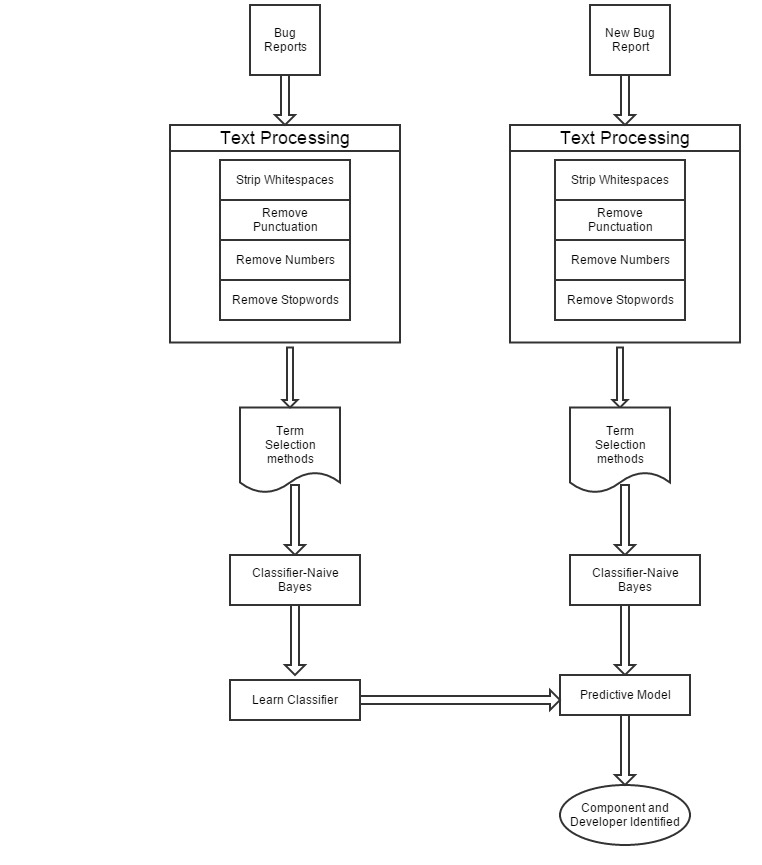
\includegraphics[height=15cm,width=15cm]{module}

\begin{figure}[hbt]
\begin{center}
\setboolean{@twoside}{false}

\includepdf[pages=12, offset =75 -75]{review3_v3.pdf}
\caption{MODULE DIAGRAM}
\end{center}
\end{figure}
%\section{Architecture Diagram}
%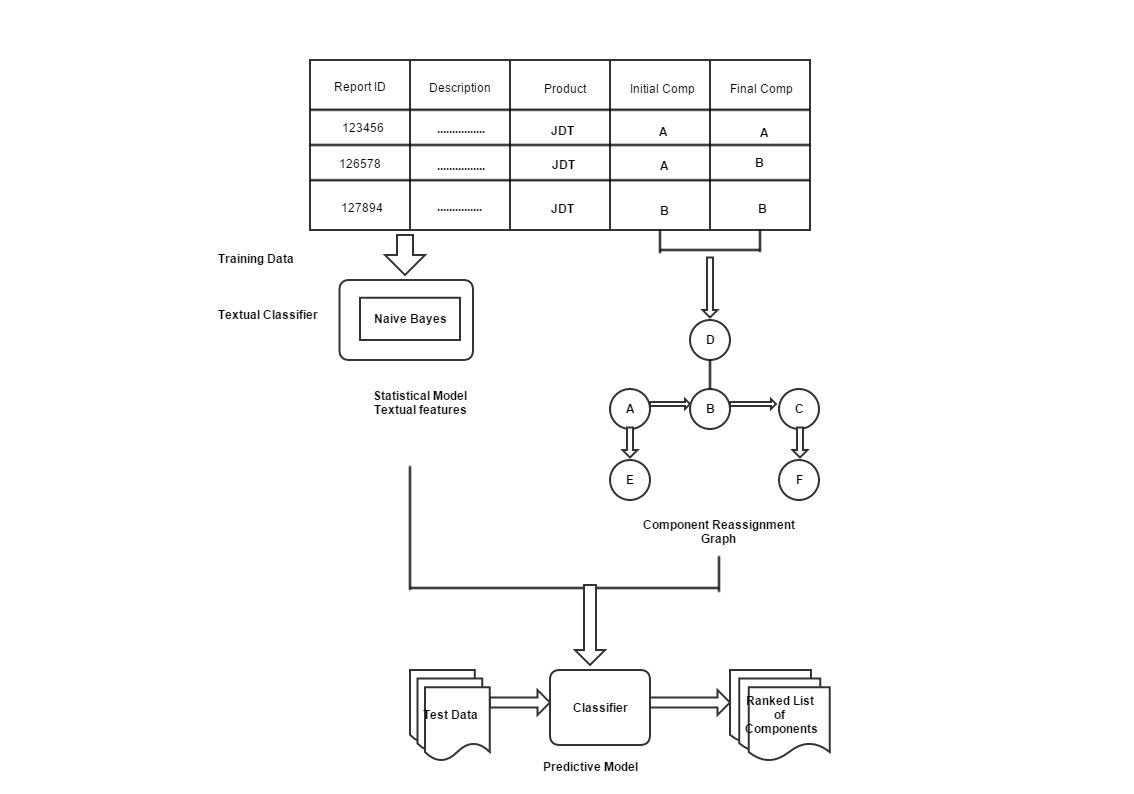
\includegraphics[height=15cm,width=17.5cm]{architecture}

%\setboolean{@twoside}{false}
%
\includepdf[left=1.5in,scale=0.8,pages=11]{review3_v3.pdf}

\newpage
\begin{figure}[hbt]
\begin{center}

\includepdf[pages=11, offset =75 -75]{review3_v3.pdf}
\caption{ARCHITECTURE DIAGRAM}
\end{center}

\end{figure}



%\section{Module Diagram}
%\begin{figure}[H]
%\input{module.pdf_tex}
%\end{figure} % LITERATURE SURVEY
% Chapter 2

\chapter{Literature Survey} % Write in your own chapter title

Cubranic et al. [1] were the first to propose the idea of using text classification methods (similar to methods used in machine learning) to semi-automate
the process of bug assignment. They used keywords extracted from the title
and description of the bug report, as well as developer ID’s as attributes, and
trained a Naive Bayes classifier. When presented with new bug reports, the
classifier suggests one or more potential developers for fixing the bug. Their
method used bug reports for Eclipse for training, and reported a prediction accuracy of up to 30\%. While we use classification as a part of our approach, in addition, we employ incremental learning and tossing graphs to reach higher accuracy.

Anvik et al. [2] improved the machine learning approach proposed by Cubranic et al. by using filters when collecting training data: (1) filtering out bug reports
labeled “invalid,” “wontfix,” or “worksforme,” (2) removing developers who no longer work on the project or do not contribute significantly, and (3) filtering developers who fixed less than 9 bugs. They used three classifiers, SVM, Naive Bayes and C4.5. They observed that SVM (Support Vector Machines) performs better than the other two classifiers and reported prediction accuracy of up to 64%.

Lin et al. [3] conducted machine learning-based bug assignment on a proprietary project, SoftPM. Their experiments were based on 2,576 bug reports. They report 77.64\% average prediction accuracy when considering module ID (the module a bug belongs to) as an attribute for training the classifier; the accuracy drops to 63\% when module ID is not used. Their finding is similar to our observation that using product-component information for classifier training improves prediction accuracy.

Jeong et al. [4] introduced the idea of using bug tossing graphs to predict
a set of suitable developers for fixing a bug. They used classifiers and tossing
graphs (Markov-model based) to recommend potential developers.

Pamela bhattacharya et al.[5] proposed a technique for automated bug assignment using machine learning and tossing graphs. They used a classifier and a tossing graph to automatically assign a bug to a developer. Initially, they used a training data set of fixed bugs that contains information regarding the developers to whom it was assigned and the reassignment to other developers.



 




 % DESIGN
% Chapter 3

\chapter{Algorithms for Automatic Bug Triaging}
The various algorithms for Automatic Bug Triaging depend on the dataset being used. The training dataset obtained after parsing, has been subjected to stop-word removal and stemming. Snowball Stemming algorithm is used for stop-word removal and stemming. Multinomial NB classifier is used for converting the data set to feature vectors. 

%\section{Algorithm}
The product, component and short description of each bug from the Training data set are parsed using a XSLT parser to obtain an unified text file. The report ID of each bug from the \texttt{assigned-to.xml} file is taken and the "when" attribute of each update of the bug is taken and matched with the corresponding entries in \texttt{short-desc.xml}, \texttt{product.xml} and \texttt{component.xml} and extracted and output to a text file in a format suitable for text processing.




\section{Snowball Stemming Algorithm}
The above parsed data has to be processed to extract the keywords. Stop-word and special Characters removal is first performed using the Natural Language ToolKit in python. Then the same Toolkit is used to perform stemming on the text after the stop-words are removed. 

\begin{algorithm}[H]
	\DontPrintSemicolon % Some LaTeX compilers require you to use \dontprintsemicolon instead
	\SetKwFunction{STEM}{STEM}
	\KwIn{$F$: Text file containing the Training dataset
	\newline $S$: Set of stop-words for the language English}
	\KwOut{$FP$ : Text file containing the Training dataset after stop-word removal and Stemming}
	\ForEach(\tcp*[h]{For each line in the file}){ line $L$ in $F$} { 
		\ForEach(\tcp*[h]{For each word in the line}){ word $W$ in $L$}{
			\If(\tcp*[h]{If the word is not a stop-word}){$W$ not in  $S$} {
		\STEM{$W$} \;
	}
	\tcc{Performs Stop-word removal and Stemming on each $W$}
		}
	
	}
	\Return{$FP$}\;
	\caption{{\sc Snowball Stemming} - Removes Stop-words and performs Stemming}
	\label{algo:Snowball Stemming}
\end{algorithm}

\section{Naive Bayes Text Classifier Algorithm}
Through supervised learning the system learns from the TDS(Training data set)- the keywords present in the description of the bug and the developer to whom it was assigned. It also gathers information about the reassignment of bugs.

The system uses Naive Bayes classifier to classify the new bugs reported, to calculate the probability of it being assigned to a developer. Naive Bayes is a probabilistic technique that uses Bayes rule of conditional probability to determine the probability that an instance belongs to a certain class. Bayes rules states that, "The probability of a class conditioned on an observation to the prior probability of the class times the probability of the observation conditioned on the class" and can be denoted as follows:

\[{P(Class|Observation)} = {\frac{P(Observation|Class)*P(Class)}{P(Observation)}}\]

For example, if the word 'concurrency' occurs more frequently in the reports resolved by developer A than in the reports resolved by developer B, the classifier would predict A as a potential fixer for a new bug report containing the word 'concurrency'. “ Naive Bayes ” is so called because it makes the strong assumption that features are independent of each other, given the label (the developer who resolved the bug).

\begin{algorithm}[H]
	\DontPrintSemicolon % Some LaTeX compilers require you to use \dontprintsemicolon instead
	\SetKwFunction{STEM}{STEM}
	\KwIn{$T$: Training corpus
	\newline $B$: New Bug Report}
	\KwOut{$d_j$ : The developer with the highest probability to whom the bug will be assigned.}
	$From\ Training\ corpus,\ extract\ Vocabulary$ \;
	\ForEach(\tcp*[h]{Calculate P($d_j$) terms}){ developer $d_j$ in $D$} { 
		$reports_j \gets {all\ bug\ reports\ in\ developer\ d_j}$ \;
		$P(d_j) \gets {\frac{|reports_j|}{|total\ no.\ reports|}}$ \;
	
	}
	$Text_j \gets {single\ text\ containing\ all\ reports_j}$ \;
\ForEach(\tcp*[h]{Calculate P($w_k | d_j$)  terms}){ word $w_k$ in $Vocabulary$} { 
		$n_k \gets {no.\ of\ occurences\ of\ w_k\ in\ Text_j}$ \;
		$P(w_k |d_j) \gets {\frac{n_k+const}{n+const|Vocabulary|}}$ \;
		
		\tcc{ $const = 1$, Laplacian Smoothing constant}
	
	}	
	
	\Return{$d_j\ with\ highest\ probability$}\;
	\caption{{\sc Naive Bayes Classifier} - Text classification}
	\label{algo:Naive Bayes}
\end{algorithm}

\section{Multinomial Naive Bayes Algorithm}
Feature Vector :
		$W$=($w_1$, $w_2$, $w_3$, ..., $w_n$)
\begin{equation}
	log\ p(D_k|W) = log\ p(D_k) + \sum\limits^{N}_{i=1}w_i\ .\ log\ p(w_i|D_k)
\end{equation}
Prior : ${\frac{|N_c|}{|N|} }$
Conditional Probability : $\frac{count(w,D_k)+1}{count(D_k)+|V|}$		
\begin{algorithm}[H]
	\DontPrintSemicolon % Some LaTeX compilers require you to use \dontprintsemicolon instead
	\SetKwFunction{STEM}{STEM}
	\KwIn{$R$: Training Corpus(List of bug reports)
	\newline $C$: List of developers}
	\KwOut{V-vocabulary,prior and condprob }
	$V \gets {\ extract\ Vocabulary}$ \;
    $N \gets {\ count\ bug\ Reports}$ \;

   
	\ForEach{ developer $d$ in $D$} 
	{     
		$N_c \gets {\ count\ bug\ reports\ in\ developer\ d\ from\ R}$ \;
    		$prior(d) \gets {\frac{|N_c|}{|N|} }$ \;
    		$words_c \gets {\ collect\ all\ words\ from\ all\ bug\ reports\ in\ developer\ c}$ \;	
    	
    		\ForEach{ word $w$ in $V$} 
    		{
    			$T_c \gets {\ count\ occurences\ of\ word(w,words_c)}$ \;
    			$T_c' \gets {\ count words(c)}$ \;
    			$condprob(w|c) \gets {\frac{|T_c+1|}{T_c' + 1 } }$ \;
    		} 
	}
	\Return{$V\ ,prior\ and\ condprob$}\;
	\caption{{\sc Train MultinomialNB} - Text classification}
	\label{algo:Train MNB}
\end{algorithm}
\newpage
\begin{algorithm}[H]
	\DontPrintSemicolon % Some LaTeX compilers require you to use \dontprintsemicolon instead
	\SetKwFunction{STEM}{STEM}
	\KwIn{$C$: List of Developers
	\newline $V$: Vocabulary
	\newline prior
	\newline condprob
	\newline $R$: Bug Report}
	\KwOut{$d$: The developer with the highest probability to whom the bug maybe assigned to.}
	$W \gets {\ extract\ words from\ Report\ R}$ \;
	\ForEach{ developer $d$ in $D$} 
	{     
    		$P(d|R) \gets {log(prior(d))}$ \;
    		\ForEach{ word $w$ in $W$} 
    		{
    			freq = count(w,R) \;
    			$P(d|R)$ += freq * log(condprob($w|d$))
	    	}
    }
	
	\Return{$argmax_d\ P(d|R)$}\;
	\caption{{\sc Apply MultinomialNB} - Text classification}
	\label{algo:Apply MNB}
\end{algorithm}

\section{Tf- idf Weight Calculation}
 Term Frequency - Inverse Document Frequency(tf-idf) is a numerical statistic that is intended to reflect how important is a word to a document in a collection or corpus. This is to minimize the frequently occurring words in all the documents(bug reports) from reducing the efficiency in bug assignment. 
\[{tf(t,doc) = 0.5 + \frac{0.5 \times f(t, doc)}{\max\{f(w, doc):w \in doc\}} }\] 
\[{ idf(t, DOC) = \log \frac{N}{1+|\{doc \in DOC: t \in doc\}|}  }\]
\[{ tfidf(t,doc,DOC) = tf(t,doc) \times idf(t, DOC)  }\]

\section{Linear Support Vector Machine}
An Support Vector Machine (SVM) is a kind of large margin classifier. It is a vector space based Machine Learning method, where the goal is to find a decision boundary between two or more classes that is maximally far from any point in the training data. An Binary SVM model is a representation of the examples as points in space, mapped so that the examples of the separate categories are divided by a clear gap that is as wide as possible.
\[{D = \left\{ (x_i, y_i)\mid x_i \in {R}^p,\, y_i \in \{ -1,1\}\right\}_{i=1}^n}\]
Multi-class SVM is implemented by reducing the single multi-class problem into multiple binary classification problems.(one-versus-all).

\section{Folding}
In folding based training and validation approach, also known as cross validation, the algorithm first collects all bug reports to be used for TDS (Training Data Set) sorts them in chronological order(based on the update time of the bug) and then divides them into \textit{n} folds. In the first run, fold 1 is used to train the classifier and then to predict the VDS (Verified Data Set). In the second run, fold 2 bug reports are added to TDS. In general, after validating the VDS from fold \textit{n}, VDS is added to the TDS for validating fold \textit{n+1}. For example, we chose \textit{n=10} and carried out 9 iterations of the validation process using incremental learning.
\newpage
%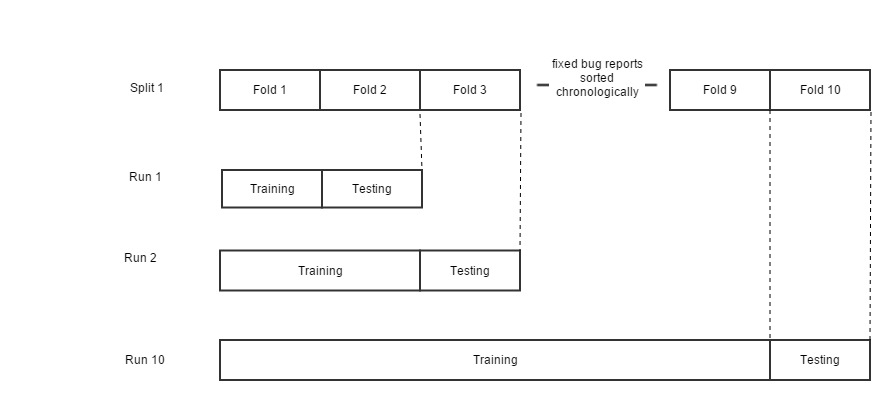
\includegraphics[height=15cm,width=15cm]{folding}
\begin{figure}[hbt]
\begin{center}

\includepdf[scale=0.8,pages={27}, offset =75 -75]{review3_v3.pdf}
\caption{FOLDING}
\end{center}
\end{figure}
\newpage

\section{Goal oriented tossing graph}
When a bug is assigned to a developer for the first time and if she is unable to fix it, the bug is assigned(tossed) to another developer. Thus a bug is tossed from one developer to another until a developer is eventually able to fix it. Based on these tossing path, goal oriented tossing graphs were proposed. Tossing graphs are weighted directed graphs such that each node represents a developer, and each directed edge from D1 to D2 represents the fact that bug is assigned to developer D1 was tossed and eventually fixed by developer D2. The weight of the edge between two developers is the probability of a toss between them, based on bug tossing history. We denote a tossing event from developer D to $D_j  as D \implies D_j$.

\newpage
\begin{table}[hbt]
\begin{center}

\includepdf[scale=0.8,pages={31}, offset =75 -75]{review3_v3.pdf}
\caption{GOAL ORIENTED TOSSING GRAPH}
\end{center}
\end{table} 

\newpage
\section{Prediction Accuracy}

If the first developer in our prediction list matches the actual developer who fixed the bug, we have a hit for the Top 1 developer count. Similarly, if the second developer in our prediction list matches the actual developer who fixed the bug, we have a hit for the Top 2 developer count. For example, if there are 100 bugs in the VDS and for 20 of those bugs the actual developer is the first developer in our prediction list, the prediction accuracy for Top 1 is 20\%; similarly, if the actual developer is in our Top 2 for
60 bugs, the Top 2 prediction accuracy is 60\%.
 % IMPLEMENTATION
% Chapter 4

\chapter{Problem Definition and Proposed System} % Write in your own chapter title


\section{Problem Statement}
\emph{Input}: A bug report in natural language text submitted by the reporter briefing the problem.\linebreak
\emph{Output}: The component in which the bug may potentially be, and the developer or list of developers to whom it can be assigned to.

When the user finds a bug, he/she reports the bug through a bug tracker used by the Software. Since the description of the bug submitted by the user is a natural language text, Natural Language Processing is used to extract useful keywords from the bug report that would provide information about the bug that the user has encountered. The processing involves stop-word removal and stemming to extract useful keywords from the description of the bug report. These extracted keywords are used to identify the most probable defective component based on the dependencies that are previously learnt. Then based on the defective Component and Tossing History of the developers, a list of Developers will be informed of this bug to solve.

The list of Developers should be chosen in such a way that the probability of the bug getting reassigned must be minimum. After fixing the bug, the bug report is annotated/labelled with the developer and the component related to the bug. A dependency structure is formed over time for supervised learning from the fixed bugs.

\section{Data Set}
Dataset is a collection of fixed bug reports gathered from a open
source software bug tracker tool containing necessary information
about the components, developers and re-assignments. This is a
categorized, classified, and semi-structured data. A bug report, generally a
natural language text, submitted by the user is stored in the XML
format by the bug tracker tool. Information contained in the dataset:
\begin{itemize}
\item \emph{severity}: The severity denotes how soon the bug should be fixed.
\item \emph{product}: The particular software application the bug is related to.
\item \emph{component}: The relevant subsystem of the product for the reported bug.
\item \emph{assigned to}: The identifier of the developer to whom the bug was assigned to.
\item \emph{short desc}: Contains a natural language text embedded by the user.
\item \emph{bug status}: The status of the bug at every update. NEW, ASSIGNED, RESOLVED, VERIFIED, REOPENED.
\item \emph{resolution}: Tagging the bug report for maintenance. FIXED, REMIND, INVALID, WORKSFORME.
\end{itemize}
With these information the dependencies between the components, developers, and reassignment can be formed.

\section{Sample Data set}

\begin{verbatim}
<report id="122442">
	<update>
    	<when>1136131494</when>
      	<what>jdt-core-inbox@eclipse.org</what>
    </update>
    <update>
      	<when>1136182552</when>
      	<what>frederic_fusier@fr.ibm.com</what>
	</update>
</report>
\end{verbatim}
A sample report in \texttt{assignedto.xml} data set.  It specifies
the developer to whom it was assigned to at every update along with the time of each update.

\begin{verbatim}
<report id="122442">
    <update>
     	<when>1136131494</when>
      	<what>API inconsistency with IJavaSearchConstants.IMPLEMENTORS and SearchPattern</what>
    </update>
    <update>
      	<when>1136182552</when>
      	<what>[search] API inconsistency with IJavaSearchConstants.IMPLEMENTORS and SearchPattern</what>
	</update>
</report>
\end{verbatim}
The short description of the bug report submitted by the reporter.

\begin{verbatim}
<report id="122442">
    <update>
      <when>1136246754</when>
      <what>Core</what>
    </update>
    <update>
      <when>1136276291</when>
      <what>UI</what>
    </update>
  </report>
\end{verbatim}
Gives information about the component involved at every update.
The bug is trivially tracked using its report-id.
\newline
\lstset{language=XML}
\begin{lstlisting}
<xsl:choose>					
	<xsl:when test="document('short_desc.xml')//short_desc/
report[@id=$w]/update[when=$x]/what!=''">
		<xsl:text>     </xsl:text>					
		<xsl:value-of select="concat('what=',document
('short_desc.xml')//short_desc/report[@id=$w]/update[when=$x]
/what,'&#10;')">
		</xsl:value-of>
	</xsl:when>
</xsl:choose>
\end{lstlisting}

First the dataset in XML format is what we used but it has only around 10000 reports. To obtain higher efficiency, we used dataset which is in JSON format it has around 1,60,000 reports in a well structured manner.
Training data set in JSON format compares the report-id and the update("when") of each report-id in the respective files and merges the "what" content present in short$\_$desc(to get the bug report) component(to obtain the component) and assigned$\_$to(the developer) to a single text file. This text file is pre-processed. The pre-processed file is converted to a feature-vector pair where the feature is the bug-report and the component it is present and the vector being the developer. The classifier learns from this feature-vector pair and predicts the accurate developer for incoming bug reports. Another feature-vector pair (component and developer) learned by the classifier is used for tossing graphs. The probability of developer solving the bug in particular component and his tossing to another developer are combined and the next probable developer who can fix the bug is determined.

\lstdefinelanguage{json}
{
	morestring=[b]",
	morestring=[d]'
}
\begin{lstlisting}[language=json,firstnumber=1]
{"assigned_to" : "123456": [{"who":86,
							  "what": Platform-UI-Inbox@eclipse.org, //developer/
							  "when":1023451345}, {"who":18,
							  "what": jhalhead@ca.ibm.com,
							  "when":10234513232} ],
				 "124323": [{"who":44,
							  "what": pde-ui-inbox@eclipse.org, 
							  "when":101234245467}, {"who":11,
							  "what": Darin_Wright@oti.com,
							  "when":102345112342} ] }			  
{"short_desc" : "123456": [{"who":86,
							  "what": Proxy Dialog when invoking Content Assist , //Short Description/
							  "when":1023451345}, {"who":18,
							  "what": Allow editing of non-project files,
							  "when":10234513232} ],
				 "124323": [{"who":44,
							  "what": content assist displays accessors, 
							  "when":101234245467}, {"who":11,
							  "what": No refresh in package view when switching internal JAR,
							  "when":102345112342} ] }
{"component" : "123456": [{"who":86,
							  "what": Core, //Component/
							  "when":1023451345}, {"who":18,
							  "what": Text,
							  "when":10234513232} ],
				 "124323": [{"who":44,
							  "what": Text, 
							  "when":101234245467}, {"who":11,
							  "what": UI,
							  "when":102345112342} ] }							  
\end{lstlisting}
After parsing, the output text file contains data in the following format:
\begin{verbatim}
JDT, Type hierarchy returns type twice if executed on working copy layer, Core
JDT, Context Menu suggests I ca run applets that doesn't exists, Debug
JDT, Identation broken when copying lines, Text
\end{verbatim} % CONCLUSION AND FUTURE WORK
% Chapter 5

\chapter{Conclusion and Future Work} % Write in your own chapter title
Machine learning and tossing graphs have proved to be promising for automating bug assignment. In this paper we lay the foundation for future work
that uses machine learning techniques to improve automatic bug assignment
by examining the impact of multiple machine learning dimensions—learning
strategy, attributes, classifiers—on assignment accuracy.
\begin{itemize}
\item We used a broad range of text classifiers and found that, like many problems which use specific machine learning algorithms, we could able to select a specific classifier for the bug assignment problem.

\item We validated our approach on two large, long-lived open-source projects; in the future, we plan to test how our current model generalizes to projects of
different scale and lifespan. In particular we would like to find if the classifier preference should change as the project evolves and how source code familiarity of a developer could be used as an additional attribute for ranking developers.

\item Similarly, when we assign tossing probabilities, we only consider the developer who could finally fix the bug. However, it is common that developers contribute
partially to the final patch in various ways. For example, when a bug is assigned
to a developer, he might provide insights and add notes to the bug report instead of actually fixing the bug; in fact, there are contributors who provide
useful discussions about a bug in the comment sections of a bug report who
are never associated with the fixing process directly. These contributions are
not considered in our ranking process,

	%Tossing graphs are weighted directed graphs such that each node represents a developer, and each directed edge from D1 to D2 represents the fact that bug assigned to developer D1 was tossed and eventually fixed by developer D2. The weight of the edge between two developers is the probability of the toss between them, based on bug tossing history.%
\end{itemize}

% Chapter 7

\chapter{Result} % Write in your own chapter title
\label{Chapter7}

\section{Experimental Set-up}
We used Mozilla and Eclipse bugs to measure the accuracy of our proposed
algorithm. We analysed the entire life span of both applications.  We divided our bug data sets into 10 folds and executed 9 iterations to cover all the folds.
Data collection. We used the bug reports to collect four kinds of data:
1. Keywords: we collect keywords from the bug description and
comments in the bug report.
2. Bug source: we retrieve the product and component the bug has been filed
under from the bug report.
3. Temporal information: we collect information about when the bug has
been reported and when it has been been fixed.
4. Developers assigned: we collect the list of developer IDs assigned to the bug

In our experiments, we varied the size of the test set, the
size of the vocabulary. The below graph shows the classification accuracy as a function of the train/test set split, when the full vocabulary
V of words found in bug reports is used.

\begin{figure}[hbt]
\begin{center}
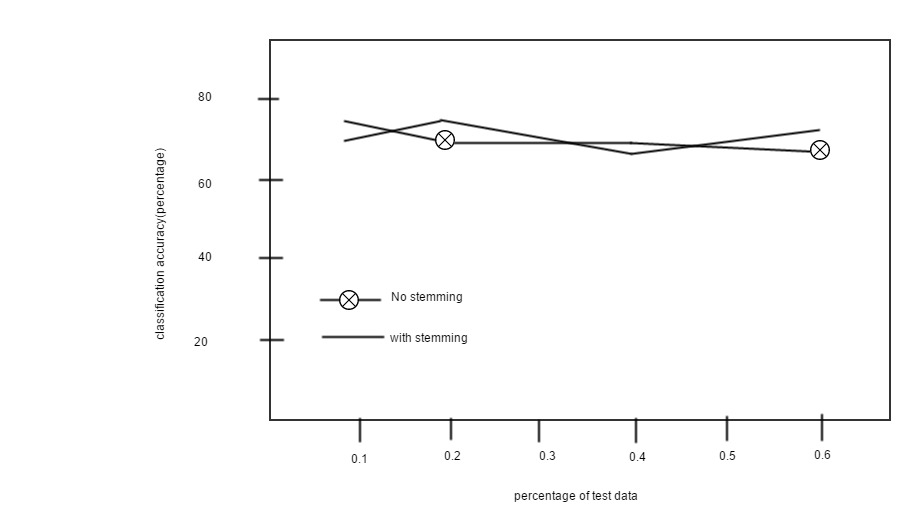
\includegraphics[height=15cm,width=15cm]{graph}
\caption{EXPERIMENTAL SET-UP}
\end{center}
\end{figure}


As we can see, the algorithm correctly assigns just under
75\% of the bugs, when 90\% of the document corpus is used
as training and 10\% as the test set. The accuracy slowly
declines to 65\% as the test set’s size is increased to 50% of
the corpus. 
\newline 

The graph also shows the results when the vocabulary was created using stemming, which identifies most grammatical variations of a word—such as “see”, “sees”, “seen”, for example—and treats them as a single term. The results are virtually unchanged, and any differences between the two conditions are within about one standard deviation at each data point.

Finally with 10 fold cross validation an accuracy of nearly 78\% is achieved and with linear SVM an accuracy of 80\% is achieved. % Result
%\chapter{Bibliography}
\begin{thebibliography}{99}
 \bibliographystyle{plain}

\bibitem[1]{icse} Anvik, J., Hiew, L., G. C. Murphy (2006), `Who should fix this bug $?$', In proc. of ICSE`06, 
pp. 361-370.

\bibitem[2]{ucr} Bhattacharyaa, P., Neamtiua, I. (2010), `Automated, Highly-Accurate, Bug Assignment Using Machine Learning and Tossing Graphs',  In proc. of ICSM`10, pp.1-10.

\bibitem[3]{seke} Cubranic, D., Murphy, G.C., (2004), `Automatic bug triage using text categorization', In proc. of SEKE`04 .

\bibitem[4]{fse} Jeong, G., Kim, S., Zimmermann, T.,  (2009), `Improving Bug Triage with Bug Tossing Graphs', In proc. of FSE`09.

\bibitem[5]{esem} Lin, Z., Shu, F., Yang,Y., Hu,C., Wang, Q., (2009), `An empirical study on bug
assignment automation using Chinese bug data', In proc. of ESEM`09.

\bibitem[6]{dataset} The Eclipse and Mozilla Defect Tracking Dataset(2013)\newline Available From: $<https://github.com/ansymo/msr2013-bug\_dataset>$.


\end{thebibliography}
 

\end{spacing}
\newpage
\appendix
%
\chapter{Infinite Mixture Models}
The use of infinite mixture models, greatly improves the desirability of flat clustering
in areas where hierarchical clustering is used if only because of the need to prespecify 
the number of clusters. In many real life data set one can only make random guesses as to
the number of clusters that are to exist. A data set may contain a skewed version of class
distribution. Infinite models intelligently guess the cluster number on the basis of the 
skew in distribution, which offer ample cues as to the non-homogeneity of the data.
Parameter-free inference in such mixture models reduce the burden
on the user by not requiring him/her to intelligently guess the parameters. The following infinite
models were discussed in this thesis.
\begin{itemize}
\item Gibbs Sampling : Gibbs sampling is intuitive and completely probabilistic. Most 
mixture models lend themselves well to conjugacy. This results in standard posterior distributions.
In the rare event that the posterior distribution is non-standard, slice sampling resolves the issue.
Gibbs sampling does not get caught in local minima unlike other deterministic algorithms. However,
the burn in period can be prohibitively large, and each cycle of iteration takes significant CPU time.
High dimensional data 
\item Variational Inference : Independence assumption in distributions allow us to define a tractable
approximate of the intractable model distribution. Also, the assumption of factorizeability results 
in the elimination of intractable coupling. With such an assumption, we can define a whole new class
of deterministic algorithms
\item Dirichlet Process : The stick breaking process allows for an infinite number of classes. A base
distribution $G$ and a concentration parameter $\alpha$ allow sampling  from 
a distribution of distributions. 
\end{itemize}

\section{Verb Clustering}

VALEX offers the 163 SCFs frequencies of 6,397 verbs in its lexicon. It offers a basic noisy lexicon
which can be smoother (add-one or linear interpolation) to produce much better cluster results. Thresholds
can be set to filter of those frequencies that do not meet it. Skewed distributions owing to the occurences
of verbs can be made right by log normalizing the frequencies. Infinite mixture models cluster the verbs
and predict the right number of verb classes in a given data set. Randomly chosen verb classes where used as
input to the clustering algorithms. The resulting verb clusters were evaluated against Levin's verb clusters
for purity and precision.

\section{Metaphor Detection}
Initializing with a seed set of metaphors that define the selectional preference of a verb to a noun and vice
versa, we expand such a 1-1 mapping to a $*$-$*$ mapping between a verb  and noun clusters. This involves 
no human supervision other than the initial seeding. The metaphors detected are evaluated agaisnt a wordnet
baseline for coverage. 

\section{Criticism}
\subsection{Limitations}
\begin{itemize}
\item The VALEX data set uses only the SCF of verbs. It pays scant attention to the frequencies of 
prepositional phrases as they are similiar in semantically related verbs. 
\item The metaphor seed set is hand fed -- not extracted from a corpus. This is because the number of verbs and their
 SCFs in VALEX crippligly is small. Any reasonable system that detects metaphors should have a wider verb coverage.
\item Metaphors are evaluated only for coverage, not quality. Qualitative evaluation require human experts
\end{itemize}

\subsection{Extension}
\begin{itemize}
\item The four different metaphor view, vis-a-vis, comparison, selectional violation, interaction and conventional
metaphor views can be taken into account to improve the quality of metaphors, though not necessarily their coverage.
\item Introduce supervision to the assignmnent of outliers to their respective clusters. This may be done using VerbNet.
\end{itemize}


%
\chapter{Infinite Mixture Models}
The use of infinite mixture models, greatly improves the desirability of flat clustering
in areas where hierarchical clustering is used if only because of the need to prespecify 
the number of clusters. In many real life data set one can only make random guesses as to
the number of clusters that are to exist. A data set may contain a skewed version of class
distribution. Infinite models intelligently guess the cluster number on the basis of the 
skew in distribution, which offer ample cues as to the non-homogeneity of the data.
Parameter-free inference in such mixture models reduce the burden
on the user by not requiring him/her to intelligently guess the parameters. The following infinite
models were discussed in this thesis.
\begin{itemize}
\item Gibbs Sampling : Gibbs sampling is intuitive and completely probabilistic. Most 
mixture models lend themselves well to conjugacy. This results in standard posterior distributions.
In the rare event that the posterior distribution is non-standard, slice sampling resolves the issue.
Gibbs sampling does not get caught in local minima unlike other deterministic algorithms. However,
the burn in period can be prohibitively large, and each cycle of iteration takes significant CPU time.
High dimensional data 
\item Variational Inference : Independence assumption in distributions allow us to define a tractable
approximate of the intractable model distribution. Also, the assumption of factorizeability results 
in the elimination of intractable coupling. With such an assumption, we can define a whole new class
of deterministic algorithms
\item Dirichlet Process : The stick breaking process allows for an infinite number of classes. A base
distribution $G$ and a concentration parameter $\alpha$ allow sampling  from 
a distribution of distributions. 
\end{itemize}

\section{Verb Clustering}

VALEX offers the 163 SCFs frequencies of 6,397 verbs in its lexicon. It offers a basic noisy lexicon
which can be smoother (add-one or linear interpolation) to produce much better cluster results. Thresholds
can be set to filter of those frequencies that do not meet it. Skewed distributions owing to the occurences
of verbs can be made right by log normalizing the frequencies. Infinite mixture models cluster the verbs
and predict the right number of verb classes in a given data set. Randomly chosen verb classes where used as
input to the clustering algorithms. The resulting verb clusters were evaluated against Levin's verb clusters
for purity and precision.

\section{Metaphor Detection}
Initializing with a seed set of metaphors that define the selectional preference of a verb to a noun and vice
versa, we expand such a 1-1 mapping to a $*$-$*$ mapping between a verb  and noun clusters. This involves 
no human supervision other than the initial seeding. The metaphors detected are evaluated agaisnt a wordnet
baseline for coverage. 

\section{Criticism}
\subsection{Limitations}
\begin{itemize}
\item The VALEX data set uses only the SCF of verbs. It pays scant attention to the frequencies of 
prepositional phrases as they are similiar in semantically related verbs. 
\item The metaphor seed set is hand fed -- not extracted from a corpus. This is because the number of verbs and their
 SCFs in VALEX crippligly is small. Any reasonable system that detects metaphors should have a wider verb coverage.
\item Metaphors are evaluated only for coverage, not quality. Qualitative evaluation require human experts
\end{itemize}

\subsection{Extension}
\begin{itemize}
\item The four different metaphor view, vis-a-vis, comparison, selectional violation, interaction and conventional
metaphor views can be taken into account to improve the quality of metaphors, though not necessarily their coverage.
\item Introduce supervision to the assignmnent of outliers to their respective clusters. This may be done using VerbNet.
\end{itemize}


%\addtotoc{REFERENCES}
%\cite{Akers78}
%\bibliographystyle{plain}

%\bibliography{ref}


\begin{thebibliography}{99}
 \bibliographystyle{plain}

\bibitem[1]{icse} Anvik, J., Hiew, L., G. C. Murphy (2006), `Who should fix this bug $?$', In proc. of ICSE`06, 
pp. 361-370.

\bibitem[2]{ucr} Bhattacharyaa, P., Neamtiua, I. (2010), `Automated, Highly-Accurate, Bug Assignment Using Machine Learning and Tossing Graphs',  In proc. of ICSM`10, pp.1-10.

\bibitem[3]{seke} Cubranic, D., Murphy, G.C., (2004), `Automatic bug triage using text categorization', In proc. of SEKE`04 .

\bibitem[4]{fse} Jeong, G., Kim, S., Zimmermann, T.,  (2009), `Improving Bug Triage with Bug Tossing Graphs', In proc. of FSE`09.

\bibitem[5]{esem} Lin, Z., Shu, F., Yang,Y., Hu,C., Wang, Q., (2009), `An empirical study on bug
assignment automation using Chinese bug data', In proc. of ESEM`09.

\bibitem[6]{dataset} The Eclipse and Mozilla Defect Tracking Dataset(2013)\newline Available From: $<https://github.com/ansymo/msr2013-bug\_dataset>$.

\end{thebibliography}


\end{document} 
